%\documentclass{uai2022} % for initial submission
 \documentclass[accepted]{uai2022} % after acceptance, for a revised
                                    % version; also before submission to
                                    % see how the non-anonymous paper
                                    % would look like
%% There is a class option to choose the math font
% \documentclass[mathfont=ptmx]{uai2022} % ptmx math instead of Computer
                                         % Modern (has noticable issues)
% \documentclass[mathfont=newtx]{uai2022} % newtx fonts (improves upon
                                          % ptmx; less tested, no support)
% NOTE: Only keep *one* line above as appropriate, as it will be replaced
%       automatically for papers to be published. Do not make any other
%       change above this note for an accepted version.

%% Choose your variant of English; be consistent
\usepackage[american]{babel}


\usepackage{natbib} % has a nice set of citation styles and commands
    \bibliographystyle{plainnat}
    \renewcommand{\bibsection}{\subsubsection*{References}}

\usepackage{import}
%%%%% start contents of packages.tex
% ICML Recommended, but optional, packages for figures and better typesetting:
\usepackage{microtype}
\usepackage{graphicx}
% \usepackage{tikz}
%\usepackage{subfigure} % Switched to floatrow + subfig
%\usepackage{booktabs} % for professional tables
% END ICML Reccomended

\usepackage{xspace} % need it for the etal/etc/eg macros. CVPR includes, ICML 
% doesn't

% \usepackage[dvipsnames]{xcolor}
\usepackage{amsmath,amssymb,amsfonts}
\usepackage{etoolbox}

\usepackage[thmmarks, amsmath, thref]{ntheorem}
\usepackage{bbm}
\usepackage{bm}

%\usepackage{ulem} % for strikethrough \sout
\usepackage[normalem]{ulem} % for \sout w/o the annoying underline in \emph

\usepackage{times}
\usepackage{epsfig}
\usepackage{graphicx}
% \usepackage{multirow}
% \usepackage{multicol}
\usepackage{xcolor}
% Subfigures
%\usepackage{subfig}
%\usepackage{floatrow}
\usepackage{subcaption}
%\floatsetup[figure]{subcapbesideposition=top}
%\floatsetup[table]{capposition=top}


% \usepackage[linesnumbered,algoruled,boxed,lined]{algorithm2e}
%  \usepackage[linesnumbered,algoruled,noend,noline]{algorithm2e}
% \usepackage[algoruled,noend,noline]{algorithm2e} % a bit shorter with no line numbers


% \usepackage{slashbox}
\usepackage{diagbox}


\usepackage{lipsum}  

\usepackage{threeparttable}
\usepackage[singlelinecheck=true,justification=centering]{caption}
\captionsetup[table]{skip=10pt}
\usepackage{makecell}
\usepackage{multirow}
\usepackage{color,soul}
\usepackage{xcolor}  

% \definecolor{battleshipgrey}{rgb}{0.52, 0.52, 0.51}
\definecolor{dimgray}{rgb}{0.35, 0.35, 0.35}

\usepackage[linesnumbered,algoruled,noend,noline]{algorithm2e}

%%%%% end contents of packages.tex

%%%%% start contents of macros.tex
 %--------------------------------------------
% Add a period to the end of an abbreviation unless there's one
% already, then \xspace.
\makeatletter
\DeclareRobustCommand\onedot{\futurelet\@let@token\@onedot}
% \def\@onedot{\ifx\@let@token.\else.\null\fi\xspace}
\def\@onedot{\ifx\@let@token.\else.\null\fi\xspace}

\def\eg{\emph{e.g}\onedot} \def\Eg{\emph{E.g}\onedot}
\def\ie{\emph{i.e}\onedot} \def\Ie{\emph{I.e}\onedot}
\def\cf{\emph{cf}\onedot} \def\Cf{\emph{Cf}\onedot}
\def\etc{\emph{etc}\onedot} \def\vs{\emph{vs}\onedot}
\def\wrt{w.r.t\onedot} 
% \def\wrt{with respect to }  % The extra space at the end means \wrt blah would 
% not end up as ``with respect toblah''. 
 
\def\dof{d.o.f\onedot}
% \def\etal{\emph{et al}\onedot}
\def\etal{\emph{et al}\onedot}
% \def\etal{\emph{et al}\onedot}
%
\def\iid{\emph{i.i.d}\onedot}
% \def\pdf{\emph{p.d.f}\onedot}



\makeatother
%--------------------------------------------------

\newcommand{\FIG}{Fig.~}
\newcommand{\FIGS}{Figs.~}
\newcommand{\EQN}{Eq.~}
% \newcommand{\EQN}{Equation }
\newcommand{\EQNS}{Eqs.~}
% \newcommand{\EQNS}{Equations }

%\newcommand{\SEC}{Sec.~}.  Use \autoref or ~\autoref instead.



% integers
\newcommand{\ZZ}{\ensuremath{\mathbb{Z}}}
\newcommand{\RR}{\ensuremath{\mathbb{R}}}
\newcommand{\Rtwo}{\ensuremath{\RR^2}}
\newcommand{\Rthree}{\ensuremath{\RR^3}}
\newcommand{\Rfive}{\ensuremath{\RR^5}}

\newcommand{\Rsix}{\ensuremath{\RR^6}}

\newcommand{\Rn}{\ensuremath{\RR^n}}
\newcommand{\Rd}{\ensuremath{\RR^d}}
\newcommand{\RD}{\ensuremath{\RR^D}}
\newcommand{\Rk}{\ensuremath{\RR^k}}

% 
%positive integers
\newcommand{\Zplus}{\ensuremath{\ZZ^+}}
%positive reals
% \newcommand{\Rplus}{\ensuremath{\RR^+}}

\newcommand{\Rnonneg}{\ensuremath{\RR_{\ge0}}}
\newcommand{\Rpos}{\ensuremath{\RR_{>0}}}


% set notation
% \newcommand{\set}[1]{\ensuremath{{\left\{#1\right\}}}}
\newcommand{\set}[1]{\ensuremath{{\{#1\}}}}
\newcommand{\tuple}[1]{\ensuremath{{(#1)}}}
\newcommand{\tupleLarge}[1]{\ensuremath{{\left(#1\right)}}}
\newcommand{\argmin}[1]{\ensuremath{\operatorname*{arg\,min}_{#1}}}
\newcommand{\argmax}[1]{\ensuremath{\operatorname*{arg\,max}_{#1}}}



\newcommand{\InnerProduct}[2]{\left\langle #1,#2 \right\rangle}

\newcommand{\norm}[1]{{{\left\|#1\right\|}}}
\newcommand{\sign}[1]{{\mathrm{sign}\left(#1\right)}}

\newcommand{\ellTwo}{\ell_2}
\newcommand{\ellTwoNorm}[1]{\norm{#1}_{\ellTwo}}
\newcommand{\ellOne}{\ell_1}




\newcommand{\MATRIX}[2][cccccccccccccccccccc]{\left[
 \begin{array}{#1}
 #2
 \end{array}
\right]}

\newcommand{\Mod}[1]{\ (\mathrm{mod}\ #1)}



% homogeneous coordinates
\newcommand{\bxh}{\widetilde{\bx}}

\newcommand{\RED}[1]{{{\color{red}{#1}}}}  
\newcommand{\BLUE}[1]{{{\color{blue}{#1}}}}
\newcommand{\GREEN}[1]{{{\color{green}{#1}}}}
\definecolor{orcgreen}{RGB}{100,150,100}
\newcommand{\ORCGREEN}[1]{{{\color{orcgreen}{#1}}}}
\newcommand{\MAGENTA}[1]{{{\color{magenta}{#1}}}}  

\definecolor{brown}{RGB}{165,42,42}
\newcommand{\BROWN}[1]{{{\color{brown}{#1}}}}



\newcommand{\FREIFELD}[1]{\textbf{\MAGENTA{[FREIFELD says: #1]}}}
\newcommand{\OR}[1]{\textbf{\ORCGREEN{[OR says: #1]}}}
% Make your own

\newcommand{\TBD}{\RED{[TBD]}}
\newcommand{\TODO}[1]{\RED{[TODO: #1]}}
\newcommand{\REPLACE}[2]{\RED{REPLACE. } \BLUE{#1} \RED{WITH. } \BLUE{#2}}



% In python: print_iterable(['\\bmdefine\\b{0}'.format(x)+'{'+x+'}' for x in 
% string.ascii_letters])

\bmdefine\ba{a}
\bmdefine\bb{b}
\bmdefine\bc{c}
\bmdefine\bd{d}
\bmdefine\be{e}
% \bmdefine\bf{f}  # Clashes with a standard command
\bmdefine\boldf{f}
\bmdefine\bg{g}
\bmdefine\bh{h}
\bmdefine\bi{i}
\bmdefine\bj{j}
\bmdefine\bk{k}
\bmdefine\bl{l}
\bmdefine\bm{m}
\bmdefine\bn{n}
\bmdefine\bo{o}
\bmdefine\bp{p}
\bmdefine\bq{q}
\bmdefine\br{r}
\bmdefine\bs{s}
\bmdefine\bt{t}
\bmdefine\bu{u}
\bmdefine\bv{v}
\bmdefine\bw{w}
\bmdefine\bx{x}
\bmdefine\by{y}
\bmdefine\bz{z}
\bmdefine\bA{A}
\bmdefine\bB{B}
\bmdefine\bC{C}
\bmdefine\bD{D}
\bmdefine\bE{E}
\bmdefine\bF{F}
\bmdefine\bG{G}
\bmdefine\bH{H}
\bmdefine\bI{I}
\bmdefine\bJ{J}
\bmdefine\bK{K}
\bmdefine\bL{L}
\bmdefine\bM{M}
\bmdefine\bN{N}
\bmdefine\bO{O}
\bmdefine\bP{P}
\bmdefine\bQ{Q}
\bmdefine\bR{R}
\bmdefine\bS{S}
\bmdefine\bT{T}
\bmdefine\bU{U}
\bmdefine\bV{V}
\bmdefine\bW{W}
\bmdefine\bX{X}
\bmdefine\bY{Y}
\bmdefine\bZ{Z}


\bmdefine\balpha{\alpha}
\bmdefine\bbeta{\beta}
\bmdefine\bgamma{\gamma}

\bmdefine\bdelta{\delta}
\bmdefine\btheta{\theta}
\bmdefine\blambda{\lambda}
\bmdefine\bphi{\phi}
\bmdefine\bxi{\xi}
\bmdefine\bzeta{\zeta}
\bmdefine\boldeta{\eta}
\bmdefine\bpi{\pi}

\bmdefine\bmu{\mu}
\bmdefine\brho{\rho}
\bmdefine\bomega{\omega}
\bmdefine\bOmega{\Omega}
\bmdefine\bPi{\Pi}

\bmdefine\bvarepsilon{\varepsilon}
\bmdefine\bepsilon{\epsilon}


\bmdefine\bDelta{\Delta}

\bmdefine\bTheta{\Theta}

\bmdefine\bsigma{\sigma}
\bmdefine\bSigma{\Sigma}
\bmdefine\bPsi{\Psi}
\bmdefine\bLambda{\Lambda}



\bmdefine\bzero{0}
\bmdefine\bone{1}
\bmdefine\binfty{\infty}

 \newcommand{\indicator}{\mathbbm{1}}


% In python 
% print_iterable(['\\newcommand{\\'+'{0}cal'.format(x)+'}{\\mathcal{'+x+'}}' 
% for x in string.ascii_uppercase])
\newcommand{\Acal}{\mathcal{A}}
\newcommand{\Bcal}{\mathcal{B}}
\newcommand{\Ccal}{\mathcal{C}}
\newcommand{\Dcal}{\mathcal{D}}
\newcommand{\Ecal}{\mathcal{E}}
\newcommand{\Fcal}{\mathcal{F}}
\newcommand{\Gcal}{\mathcal{G}}
\newcommand{\Hcal}{\mathcal{H}}
\newcommand{\Ical}{\mathcal{I}}
\newcommand{\Jcal}{\mathcal{J}}
\newcommand{\Kcal}{\mathcal{K}}
\newcommand{\Lcal}{\mathcal{L}}
\newcommand{\Mcal}{\mathcal{M}}
\newcommand{\Ncal}{\mathcal{N}}
\newcommand{\Ocal}{\mathcal{O}}
\newcommand{\Pcal}{\mathcal{P}}
\newcommand{\Qcal}{\mathcal{Q}}
\newcommand{\Rcal}{\mathcal{R}}
\newcommand{\Scal}{\mathcal{S}}
\newcommand{\Tcal}{\mathcal{T}}
\newcommand{\Ucal}{\mathcal{U}}
\newcommand{\Vcal}{\mathcal{V}}
\newcommand{\Wcal}{\mathcal{W}}
\newcommand{\Xcal}{\mathcal{X}}
\newcommand{\Ycal}{\mathcal{Y}}
\newcommand{\Zcal}{\mathcal{Z}}


 \newcommand{\DP}{\mathrm{DP}}
 \newcommand{\DIR}{\mathrm{Dir}}

%%%%% end contents of macros.tex


\usepackage{booktabs}
%%%%%%%%%%%%%%%%%%%%%%%%%%%%%%%%%%%%%%%%%%%%%%%%%%%%%%%%%%%%%%%%%%%%%%%%%5
% Oren says:
% Load hyperref as the last package. You will live longer (and will have less warnings)
% \usepackage[colorlinks=true,    % declare we want color links
% 	    bookmarksopen=true,  % expanded bookmarks
% 	    pagebackref=false,        % or backref
% 	    linkcolor=blue,
% 	    urlcolor  = blue
% 	    ]{hyperref}
% \usepackage[backref, colorlinks,citecolor=blue]{hyperref}
% \usepackage[backref]{hyperref}
% \hypersetup{urlcolor=blue, colorlinks=true} 
\hypersetup{
  colorlinks   = true, %bColours links instead of ugly boxes
  urlcolor     = blue, %Colour for external hyperlinks
  linkcolor    = blue, %Colour of internal links
  citecolor   = blue, %Colour of citations
}

% \hypersetup{citecolor=blue}

% \usepackage{capt-of}
% \hypersetup{citecolor=blue}   
\usepackage{ellipsis} % The comment about regarding hyperref is more of a guideline than a rule... 
                      %``Note that ellipsis must be loaded after hyperref. 
                      %(The ellipsis documentation doesn't mention this, but the hyperref README does.)''

 \hypersetup{final}  % The things you learn the hard way: when draft mode is on (in \documentclass)
                     % Then the links created by hyperref are tuned off. Even if I pass draft=false and final=true to hyperref.
                     % The hypersetup{final} makes sure we have links active even in draft mode.
%   \hypersetup{draft}
               
% To have short pointers for sections and subsections. Oren Freifeld
\renewcommand{\sectionautorefname}{\S} 
\renewcommand{\subsectionautorefname}{\S} 
\renewcommand{\subsubsectionautorefname}{\S} 

\renewcommand{\algorithmautorefname}{Algorithm}
% \renewcommand{\algorithmautorefname}{Alg.~}
\newcommand{\Exampleautorefname}{Example}



\title{Variational- and Metric-based Deep Latent Space \\ for Out-of-Distribution Detection\\ -- Supplementary Material}


% The standard author block has changed for UAI 2022 to provide
% more space for long author lists and allow for complex affiliations
%
% All author information is authomatically removed by the class for the
% anonymous submission version of your paper, so you can already add your
% information below.
%
% Add authors
\author[1]{\href{mailto:<dinari@post.bgu.ac.il >?Subject=Your UAI 2022 paper}{Or Dinari}{}}
\author[1]{\href{mailto:<orenfr@cs.bgu.ac.il >?Subject=Your UAI 2022 paper}{Oren Freifeld}{}}
% Add affiliations after the authors
\affil[1]{%
    The Department of Computer Science,
    Ben-Gurion University of the Negev\\
    Be'er Sheva, Israel
}



\begin{document}
\maketitle
\onecolumn

\begin{abstract}
This document contains the following: 
1) the mathematical formulation of the KL loss;
2) the  technical details of our experiments, including the values of the hyperparameters that we used, and the details for the training of the deep nets; 
3) results on each benchmark in the OOD-detection task (in the paper we reported only the average results across those benchmarks); 
4) empirical evaluation of different features for the reconstruction weighting;  
5) details regarding the datasets used in the paper; 
6) implementation and hardware details;
7) an intuitive explanation for the effect of the overall proposed loss; 
8) details of the auto-encoders used for the reconstruction step.
\end{abstract}

\section{The Gaussian Class-conditioned KL Divergence Loss}
Let $q= \Ncal(\mu_1,\sigma_1^2)$ and $p=\Ncal(\mu_2,\sigma_2^2)$ be two univariate Gaussian distributions and let $D_{\mathrm{KL}}(\cdot||\cdot) $ denote the KL divergence.
Then: 
\begin{align}
    &D_{\mathrm{KL}}(q||p) = \int q(z)\log\left(\frac{q(z)}{p(z)}\right) \,dz
    \\ &= \int \left[\log( q(z)) - \log( p(z)) \right] q(z) \,dz\\
    &=\int \left[ -\frac{1}{2} \log(2\pi) - \log(\sigma_1) - \frac{1}{2} \left(\frac{z-\mu_1}{\sigma_1}\right)^2 + \frac{1}{2}\log(2\pi) + \log(\sigma_2) + \frac{1}{2} \left(\frac{z-\mu_2}{\sigma_2}\right)^2  \right] \nonumber \\
    &
    \quad
    \times \frac{1}{\sqrt{2\pi}\sigma_1} \exp\left[-\frac{1}{2}\left(\frac{z-\mu_1}{\sigma_1}\right)^2\right] dz\\
    &=\int \left\{\log\left(\frac{\sigma_2}{\sigma_1}\right) + \frac{1}{2} \left[ \left(\frac{z-\mu_2}{\sigma_2}\right)^2 - \left(\frac{z-\mu_1}{\sigma_1}\right)^2 \right] \right\}
%     \\
%     &
    \times 
    \frac{1}{\sqrt{2\pi}\sigma_1} \exp\left[-\frac{1}{2}\left(\frac{z-\mu_1}{\sigma_1}\right)^2\right] dz\\
    &=E \left\{\log\left(\frac{\sigma_2}{\sigma_1}\right) + \frac{1}{2} \left[ \left(\frac{z-\mu_2}{\sigma_2}\right)^2 - \left(\frac{z-\mu_1}{\sigma_1}\right)^2 \right]\right\}  \qquad \text{(the expectation is \wrt  $q$ )}
    \\
    &=\log\left(\frac{\sigma_2}{\sigma_1}\right) + \frac{1}{2\sigma_2^2} E \left\{(X-\mu_2)^2\right\} - \frac{1}{2\sigma_1^2} E \left\{(X-\mu_1)^2\right\} \\
     &=\log\left(\frac{\sigma_2}{\sigma_1}\right) + \frac{1}{2\sigma_2^2} E \left\{(X-\mu_2)^2\right\} - \frac{1}{2\sigma_1^2}  \sigma_1^2 \\
    &=\log\left(\frac{\sigma_2}{\sigma_1}\right) + \frac{1}{2\sigma_2^2} E \left\{(X-\mu_2)^2\right\} - \frac{1}{2}\\ 
    &=\log\left(\frac{\sigma_2}{\sigma_1}\right) + \frac{1}{2\sigma_2^2}\left[E\left\{(X-\mu_1)^2\right\} + 2(\mu_1-\mu_2)\underbrace{E\left\{X-\mu_1\right\}}_{0} + (\mu_1-\mu_2)^2\right] - \frac{1}{2}\\
    &=\log\left(\frac{\sigma_2}{\sigma_1}\right) + \frac{\sigma_1^2 + (\mu_1-\mu_2)^2}{2\sigma_2^2} - \frac{1}{2}\, . \label{eqn:kl}
\end{align}
Now recall our KL loss term is
\begin{align}
    \Lcal_\mathrm{KL}(\bx_i) &= -D_{\mathrm{KL}}(q(\cdot|\bg(\bx_i))||p(\cdot|y_i))
\end{align}
where 
{$q(\cdot|\bg(\bx_i))$} is a $d$-dimensional Gaussian probability density function
(pdf) with a  mean vector $\bmu(\bg(\bx_i))$ and a diagonal covariance matrix
whose $(j,j)$ entry is $\sigma_j^2(\bg(\bx_i))$
while 
%\REPLACE{$p(\boldf(\bg(\bx_i))|y_i)$}
{$p(\cdot|y_i)$} is an isotropic $d$-dimensional Gaussian pdf, associated with class $y_i$, with a mean vector $\bm(y_i)=(m_1(y_i),\ldots,m_d(y_i))$ and variance $s^2$. 
Note that both $\bq$ and $\bp$ are $d$-dimensional multivariate Gaussians 
and each of them has a diagonal covariance matrix. It follows that
\begin{align}
    D_{\mathrm{KL}}(q(\cdot|\bg(\bx_i))||p(\cdot|y_i))=\sum\nolimits_{j=1}^d  D_{\mathrm{KL}}(q_j(\cdot|\bg(\bx_i))||p_j(\cdot|y_i))
\end{align}
where $q_j(\cdot|\bg(\bx_i))$ and $p_j(\cdot|y_i)$ are the univariate Gaussians $\Ncal(\mu_j(\bg(\bx_i)),\sigma_j^2(\bg(\bx_i)))$ and $\Ncal(m_j(y_i),s^2)$, respectively. 
Putting it altogether, we obtain that:
\begin{align}
&D_{\mathrm{KL}}(q(\cdot|\bg(\bx_i))||p(\cdot|y_i)) \\ \nonumber
&=\sum\nolimits_{j=1}^d \log\left(\frac{s}{\sigma_j(\bg(\bx_i))}\right) + \frac{\sigma_j^2(\bg(\bx_i)) + (\mu_j(\bg(\bx_i))-m_j(y_i))^2}{2s^2} - \frac{1}{2}\, .
\end{align}
Finally, using the above term in the loss function results in the following expression:
\begin{align}
    \Lcal_\mathrm{KL}(\bx_i) &= -D_{\mathrm{KL}}(q(\cdot|\bg(\bx_i))||p(\cdot|y_i)) \\ \nonumber
    &= \sum\nolimits_{j=1}^d \left[-\log\left(\tfrac{s}{\sigma_j(\bg(\bx_i))}\right)-\frac{\sigma_j^2(\bg(\bx_i))+(\mu_j(\bg(\bx_i))-m_j(y_i))^2}{2s^2}+0.5\right]\, .
\end{align}

\begin{table}[t]
    \centering
    \caption{Experiments hyperparameters.}
        \label{Tab:hyper}
    \hspace*{-1cm} 
    \resizebox{\columnwidth}{!}{
    \begin{tabular}{@{}llccccccccc@{}}
    \toprule
    Dataset                   & Backbone       & $d$ & $k$ & $M_d$ & $M_t$ & Optimizer & $B_c$ & $B_n$ & $LR$  &Finetune $LR$\\ \midrule
%     \multirow{3}{*}{CIFAR-10}
    CIFAR-10
    & VGG~\citep{Yoshihashi:CVPR:2019:classification}            & 32  & 1024& 32    &  0.1  &  Adam     &  8   &  40   &  0.001&N/A           \\
           CIFAR-10                  & ResNet18~\citep{He:CVPR:2016deep}       & 32  & 512 & 32    &  0.1  &  SGD      &  10   &  40   &  0.01 &N/A           \\
            CIFAR-10                  & ResNet34~\citep{He:CVPR:2016deep}       & 32  & 512 & 32    &  0.1  &  SGD      &  10   &  8   &  0.005 &N/A           \\
      CIFAR-10                        & DenseNet-BC100~\citep{Huang:2017:densely} & 32  & 342 & 32    &  0.1  &  SGD      &  10   &  40   &  0.1 &N/A           \\
      CIFAR-10                        & WideResnet28~\citep{Zagoruyko:arxiv:2016:wide} & 32  & 640 & 32    &  0.1  &  SGD      &  10   &  20   &  0.001 &0.01           \\
    CIFAR-100                 & DenseNet-BC100~\citep{Huang:2017:densely} & 64  & 342 & 64    &  0.1  &  SGD      &  20   &  20   &  0.0001&0.01         \\
    MNIST                     & CNN~\citep{Yoshihashi:CVPR:2019:classification}            & 32  & 500 & 32    &  0.1  &  Adam     &  10   &  64   &  0.0001&N/A           \\ \bottomrule
    \end{tabular}
    }
    \end{table}


\section{Experiments Details}
Each of the well-known datasets, CIFAR10 and MNIST, comes with a partition to training data and test data. 
For our training we have only used the training data. The test data was used for only evaluation. 

\textbf{hyperparameters.}
All the training hyperparameters appear in~\autoref{Tab:hyper}.
Recall, from the paper, that we trained our model 
on each of the following pairs of dataset/backbone:
\begin{enumerate}
 \item MNIST \& CNN;
 \item CIFAR10 \& VGG;
 \item CIFAR10 \& ResNet18;
 \item CIFAR10 \& ResNet34;
  \item CIFAR10 \& DenseNet-BC100;
 \item CIFAR10 \& WideResnet28.
 \item CIFAR100 \& DenseNet-BC100. 
\end{enumerate}
Moreover, and as was also stated in the paper, in five of these cases
we trained the model from scratch, while only in the (CIFAR100, DenseNet-BC100) and (CIFAR10, WideResnet28)
pairs we merely fine-tuned a pre-trained Deep Neural Net (DNN).
Thus, in~\autoref{Tab:hyper}, the learning rate (LR) for the fine tuning
appears only in the row that corresponds to such a pair. 

We emphasize, and as was mentioned in the main text, that in our method (regardless if we train a model from scratch or if take a pre-trained model
and fine tune it for our tasks) there are no parameters that are learned/tuned 
using OOD data. 
Particularly, the only hyperparameters are standard training parameters, as described in \autoref{Tab:hyper}, while the weights of the DNN are learned using only 
data from the known classes, not OOD data. 
\subsection{Training Details for the Five Cases Where the Training was Done from Scratch}
In these experiments we used $M_d$ warm-up rounds (where the value of $M_d$ appears in~\autoref{Tab:hyper}),
where we gradually increased the distancing margin from 0.15 to $M_d$. 
While this warm-up stage is optional, we found that it increases the stability of the training. In addition,
we have started with $B'_s = B_s/5$ for the first 150 epochs. This step too is optional, but it improves the convergence speed. We reduced the LR by a factor of $\frac{1}{10}$ every 100 epochs. The total number of epochs was 500 epochs.
\subsection{Training Details for the Two Cases Where We Fine-tuned a Pre-trained DNN} 
For the fine-tuning experiments (\ie, CIFAR-100 with the DenseNet backbone and CIFAR-10 with the WideResnet28 backbone),
we have loaded the pre-trained weights from~\citep{Liang:ICLR:2018:ODIN} for CIFAR100, or first trained a SoftMax-based classifier for CIFAR10 and then loaded its weights.
Then, using the `Finetune LR' (\autoref{Tab:hyper}) we have trained the $\bmu$ and $\bsigma$ layers for (only) 20 epochs. Next, we unfroze the entire network, and continued training for additional 130 epochs,
with two LR decreases, each after 64 epochs, starting from `LR' (\autoref{Tab:hyper}).\\

\subsection{Data Augmentation}
We have used standard random augmentations during training. Specifically, 
for the MNIST experiments we have used random rotations and random resized crops.
For the CIFAR experiments we have used random crops and random horizontal flips.
% The random augmentations were followed by normalization  . \\


\subsection{Feature Ensembles}
As noted in the main text,
for block-based networks (such as DenseNet or ResNet) we used the output of the first three blocks for $(t_1,t_2,t_3)$.
For the non-block based networks that we used in the experiments (\ie, VGG and the plain CNN), we have chosen the following features:
For VGG, we have taken the outputs of the second, fourth, and eight convolution layer, each after Batch Norm and ReLU.
For the plain CNN, we have used the outputs of the second, third and fourth convolution layers.



\begin{table}[t]
    \setlength\tabcolsep{4pt}
    \centering
    \caption{ODIN~\citep{Liang:ICLR:2018:ODIN} OOD Benchmarks}
        \label{Tab:ood_odin}
         
        \begin{tabular}{@{}lllll@{}}
            \toprule
                                      & \multicolumn{2}{c}{CIFAR-10}      & \multicolumn{2}{c}{CIFAR-100}     \\ \midrule
                                      & \textit{AUROC} & \textit{TNR@TPR95} & \textit{AUROC} & \textit{TNR@TPR95} \\\midrule
            \textit{ImageNet-Crop}    & 0.991          & 0.957            & 0.945          & 0.731            \\
            \textit{ImageNet-Resize}  & 0.985          & 0.925            & 0.855          & 0.430            \\
            \textit{LSUN-Crop}        & 0.979          & 0.962            & 0.968          & 0.814            \\
            \textit{LSUN-Resize}      & 0.992          & 0.937            & 0.871          & 0.420            \\ \bottomrule
        \end{tabular}

        
        \caption{ODIN*~\citep{Hsu:CVPR:2020:generalized} OOD Benchmarks}
        \label{Tab:ood_odin_star}
        
        \begin{tabular}{@{}lllll@{}}
            \toprule
            \textit{In-distribution} & \multicolumn{2}{c}{CIFAR-10}      & \multicolumn{2}{c}{CIFAR-100}     \\ \midrule
            \textit{OOD}              & \textit{AUROC} & \textit{TNR@TPR95} & \textit{AUROC} & \textit{TNR@TPR95} \\\midrule
            \textit{ImageNet-Crop}    &  0.882         & 0.478            & 0.905          &  0.560           \\
            \textit{ImageNet-Resize}  &  0.901         & 0.519            & 0.911          &  0.594           \\
            \textit{LSUN-Crop}        &  0.913         & 0.635            & 0.899          &  0.530           \\
            \textit{LSUN-Resize}      &  0.923         & 0.592            & 0.930          &  0.640           \\ \bottomrule
        \end{tabular}
    \end{table}



\begin{table}[t]
    \setlength\tabcolsep{4pt}
    \centering
    \caption{Mahalanobis~\citep{Lee:NIPS:2018:simple} OOD Benchmarks}
        \label{Tab:ood_mahalanobis}
         
        \begin{tabular}{@{}lllll@{}}
            \toprule
                                      & \multicolumn{2}{c}{CIFAR-10}      & \multicolumn{2}{c}{CIFAR-100}     \\ \midrule
                                      & \textit{AUROC} & \textit{TNR@TPR95} & \textit{AUROC} & \textit{TNR@TPR95} \\\midrule
            \textit{ImageNet-Crop}    & 0.998          &  0.997           & 0.996          & 0.998            \\
            \textit{ImageNet-Resize}  & 0.988          &  0.952           & 0.974          & 0.866            \\
            \textit{LSUN-Crop}        & 0.996          &  0.996           & 0.993          & 0.982            \\
            \textit{LSUN-Resize}      & 0.992          &  0.973           & 0.982          & 0.914            \\ \bottomrule
        \end{tabular}

        
        \caption{Mahalanobis*~\citep{Hsu:CVPR:2020:generalized} OOD Benchmarks}
        \label{Tab:ood_mahalanobis_star}
        
        \begin{tabular}{@{}lllll@{}}
            \toprule
            \textit{In-distribution} & \multicolumn{2}{c}{CIFAR-10}      & \multicolumn{2}{c}{CIFAR-100}     \\ \midrule
            \textit{OOD}              & \textit{AUROC} & \textit{TNR@TPR95} & \textit{AUROC} & \textit{TNR@TPR95} \\\midrule
            \textit{ImageNet-Crop}    & 0.963          & 0.812            &   0.924        & 0.635            \\
            \textit{ImageNet-Resize}  & 0.982          & 0.909            &   0.964        & 0.820            \\
            \textit{LSUN-Crop}        & 0.922          & 0.642            &   0.812        & 0.316            \\
            \textit{LSUN-Resize}      & 0.982          & 0.917            &   0.966        & 0.826            \\ \bottomrule
        \end{tabular}
    \end{table}




\begin{table}[t]
    \setlength\tabcolsep{4pt}
    \centering
    \caption{DeConf-C~\citep{Hsu:CVPR:2020:generalized} OOD Benchmarks}
        \label{Tab:ood_deconf}
         
        \begin{tabular}{@{}lllll@{}}
            \toprule
                                      & \multicolumn{2}{c}{CIFAR-10}      & \multicolumn{2}{c}{CIFAR-100}     \\ \midrule
                                      & \textit{AUROC} & \textit{TNR@TPR95} & \textit{AUROC} & \textit{TNR@TPR95} \\\midrule
            \textit{ImageNet-Crop}    &  0.987         &  0.934           & 0.976          & 0.878            \\
            \textit{ImageNet-Resize}  &  0.991         &  0.958           & 0.986          & 0.933            \\
            \textit{LSUN-Crop}        &  0.983         &  0.915           & 0.953          & 0.750            \\
            \textit{LSUN-Resize}      &  0.994         &  0.976           & 0.987          & 0.938            \\ \bottomrule
        \end{tabular}
    \end{table}




\begin{table}[t]
    \setlength\tabcolsep{4pt}
    \centering
    \caption{CSI~\citep{Tack:NIPS:2020:csi} OOD Benchmarks}
        \label{Tab:ood_csi}
         
        \begin{tabular}{@{}lllll@{}}
            \toprule
                                      & \multicolumn{2}{c}{CIFAR-10}      & \multicolumn{2}{c}{CIFAR-100}     \\ \midrule
                                      & \textit{AUROC} & \textit{TNR@TPR95} & \textit{AUROC} & \textit{TNR@TPR95} \\\midrule
            \textit{ImageNet-Crop}    & 0.982          & 0.900            & 0.966          & 0.805            \\
            \textit{ImageNet-Resize}  & 0.978          & 0.875            & 0.839          & 0.284            \\
            \textit{LSUN-Crop}        & 0.987          & 0.944            & 0.974          & 0.849            \\
            \textit{LSUN-Resize}      & 0.978          & 0.870            & 0.871          & 0.388            \\ \bottomrule
        \end{tabular}
    \end{table}

    



\begin{table}
    \setlength\tabcolsep{4pt}
    \centering
    \caption{SubSpaces~\citep{Zaeemzadeh:CVPR:2021:out} OOD Benchmarks}
        \label{Tab:ood_subspaces}
         
        \begin{tabular}{@{}lllll@{}}
            \toprule
                                      & \multicolumn{2}{c}{CIFAR-10}      & \multicolumn{2}{c}{CIFAR-100}     \\ \midrule
                                      & \textit{AUROC} & \textit{TNR@TPR95} & \textit{AUROC} & \textit{TNR@TPR95} \\\midrule
            \textit{ImageNet-Crop}    & 0.981          &  0.910             & 0.891          &  0.583           \\
            \textit{ImageNet-Resize}  & 0.985          &  0.924             & 0.940          &  0.706           \\
            \textit{LSUN-Crop}        & 0.994          &  0.972             & 0.936          &  0.612           \\
            \textit{LSUN-Resize}      & 0.993          &  0.966             & 0.960          &  0.797           \\ \bottomrule
        \end{tabular}
    \end{table}
    


\begin{table}[t]
    \setlength\tabcolsep{4pt}
    \centering
    \caption{\textbf{VMDLS}$_\bb$ OOD Benchmarks}
        \label{Tab:ood_vmdls}
         
        \begin{tabular}{@{}lllll@{}}
            \toprule
                                      & \multicolumn{2}{c}{CIFAR-10}      & \multicolumn{2}{c}{CIFAR-100}     \\ \midrule
                                      & \textit{AUROC} & \textit{TNR@TPR95} & \textit{AUROC} & \textit{TNR@TPR95} \\\midrule
            \textit{ImageNet-Crop}    & 0.989          & 0.999            & 0.997          & 0.998            \\
            \textit{ImageNet-Resize}  & 0.961          & 0.953            & 0.949          & 0.748            \\
            \textit{LSUN-Crop}        & 0.991          & 0.999            & 0.996          & 0.999            \\
            \textit{LSUN-Resize}      & 0.967          & 0.972            & 0.961          & 0.768            \\ \bottomrule
        \end{tabular}

        \caption{\textbf{VMDLS} OOD Benchmarks}
        \label{Tab:ood_vmdlsp}
        
        \begin{tabular}{@{}lllll@{}}
            \toprule
            \textit{In-distribution} & \multicolumn{2}{c}{CIFAR-10}      & \multicolumn{2}{c}{CIFAR-100}     \\ \midrule
            \textit{OOD}              & \textit{AUROC} & \textit{TNR@TPR95} & \textit{AUROC} & \textit{TNR@TPR95} \\\midrule
            \textit{ImageNet-Crop}    & 0.997          & 0.999            & 0.999          & 0.999            \\
            \textit{ImageNet-Resize}  & 0.985          & 0.959            & 0.987          & 0.946            \\
            \textit{LSUN-Crop}        & 0.991          & 0.999            & 0.999          & 0.999            \\
            \textit{LSUN-Resize}      & 0.988          & 0.973            & 0.994          & 0.973            \\ \bottomrule
        \end{tabular}
    \end{table}
    
    
\section{OOD Benchmarks}
In this section we provide the full results of the OOD benchmarks.
The results for each method are shown in its own table:
ODIN in \autoref{Tab:ood_odin}; 
ODIN* in \autoref{Tab:ood_odin_star};
Mahalanobis in \autoref{Tab:ood_mahalanobis};
Mahalanobis* in \autoref{Tab:ood_mahalanobis_star};
DeConf-C in \autoref{Tab:ood_deconf};
CSI in \autoref{Tab:ood_csi};
SubSpaces in \autoref{Tab:ood_subspaces};
\textbf{VDMLS}$_\bb$ (ours) in \autoref{Tab:ood_vmdls};
\textbf{VDMLS} (ours) in \autoref{Tab:ood_vmdlsp};
Each such table shows the results, where the in-distribution data
is either CIFAR10 or CIFAR100, using one of four different OOD datasets.
The reported numbers in these seven tables stand for the macro-average results across those four OOD datasets.


\section{Empirical Evaluation of the Reconstruction Features}

\begin{figure}[ht]
    \centering
    \subcaptionbox{Unmodified values (\textbf{VMDLS}$_\bb$)}[.49\linewidth]{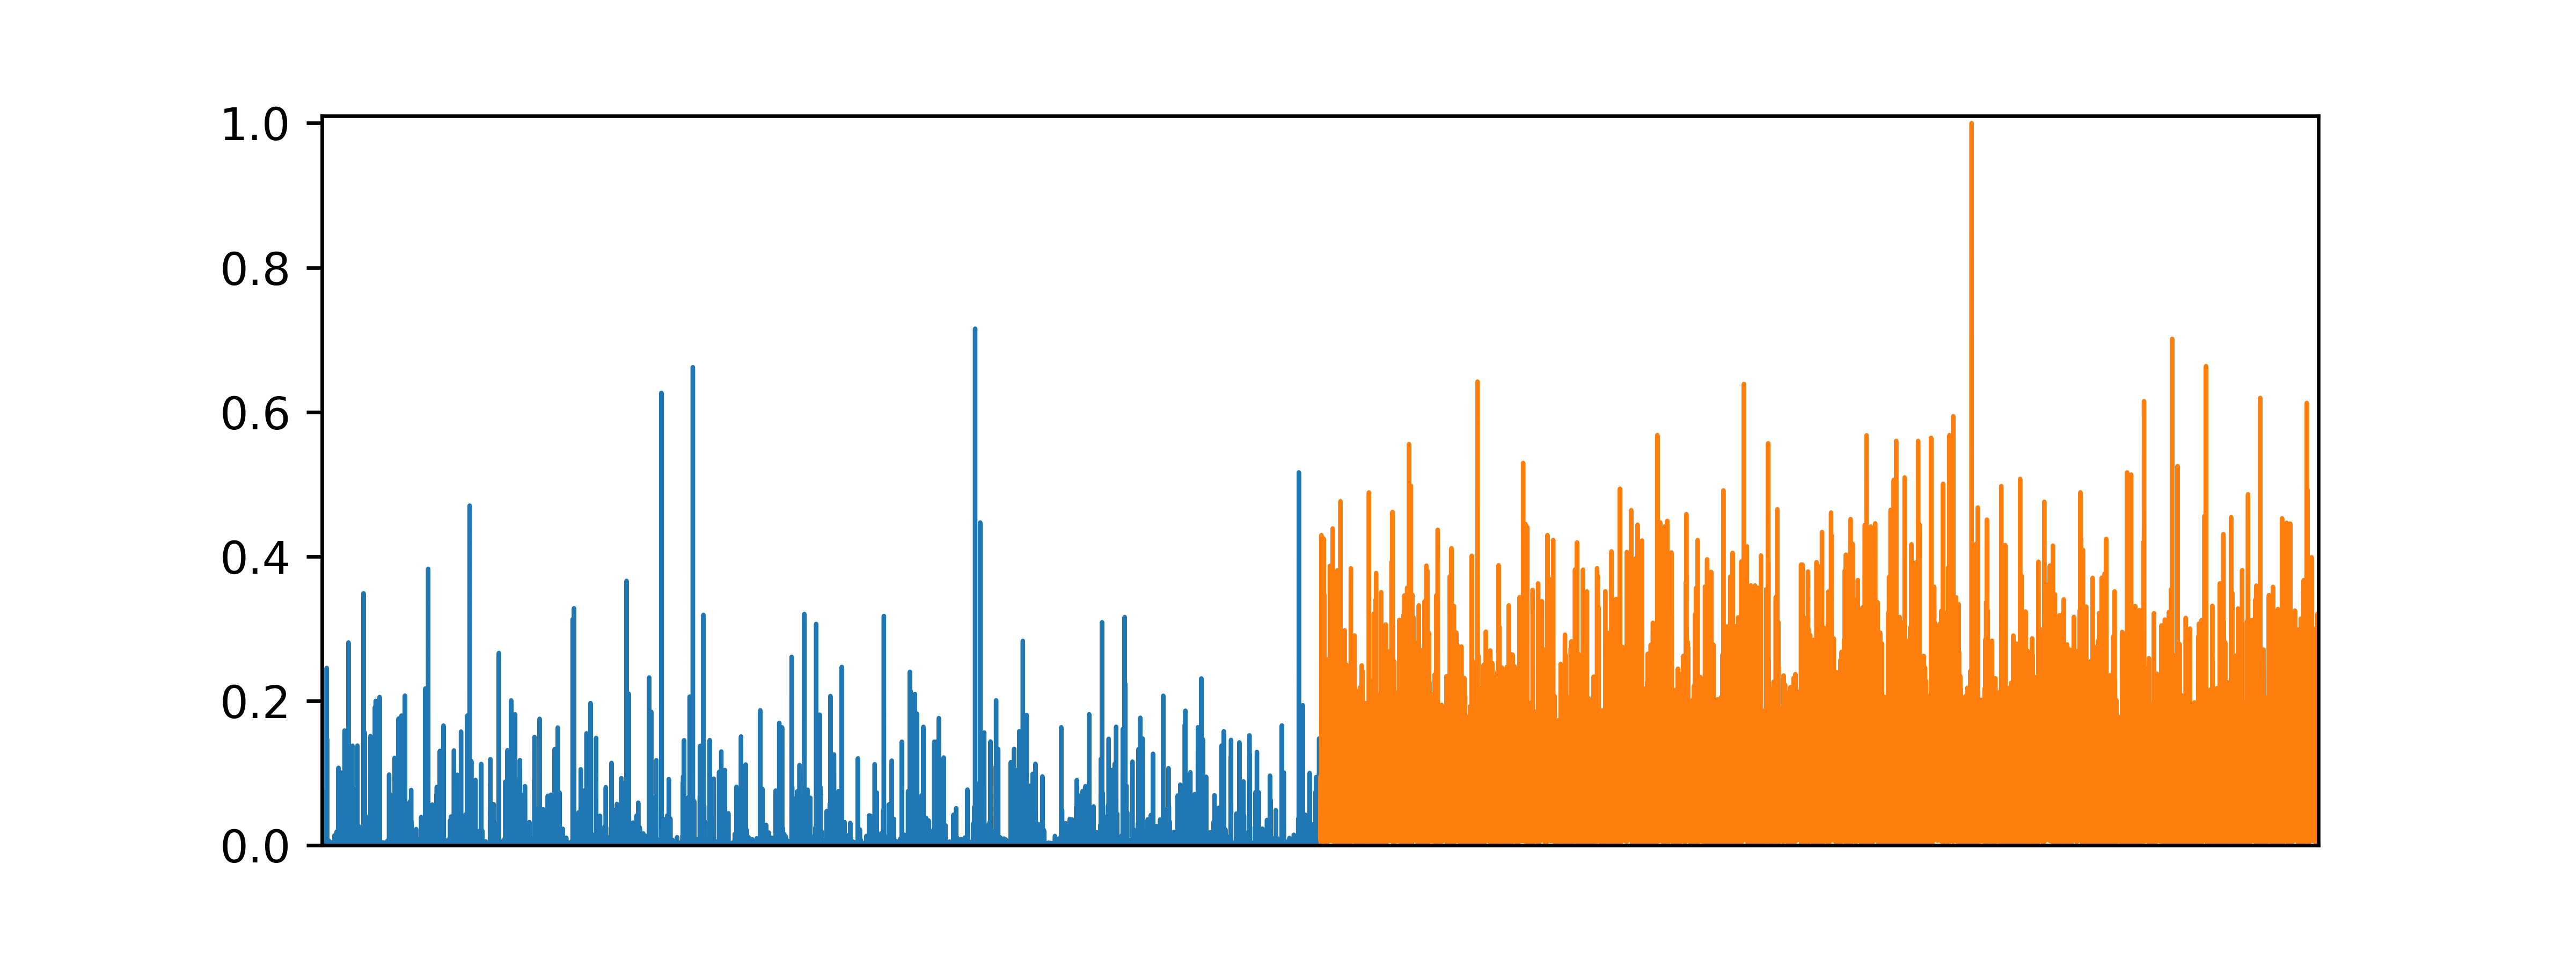
\includegraphics[height=3cm,trim=1.5cm 0.0cm 0.0cm 0.7cm,clip]{pre_ae_features.png}} 
    \subcaptionbox{Low-level features (\textbf{VMDLS})}[.49\linewidth]{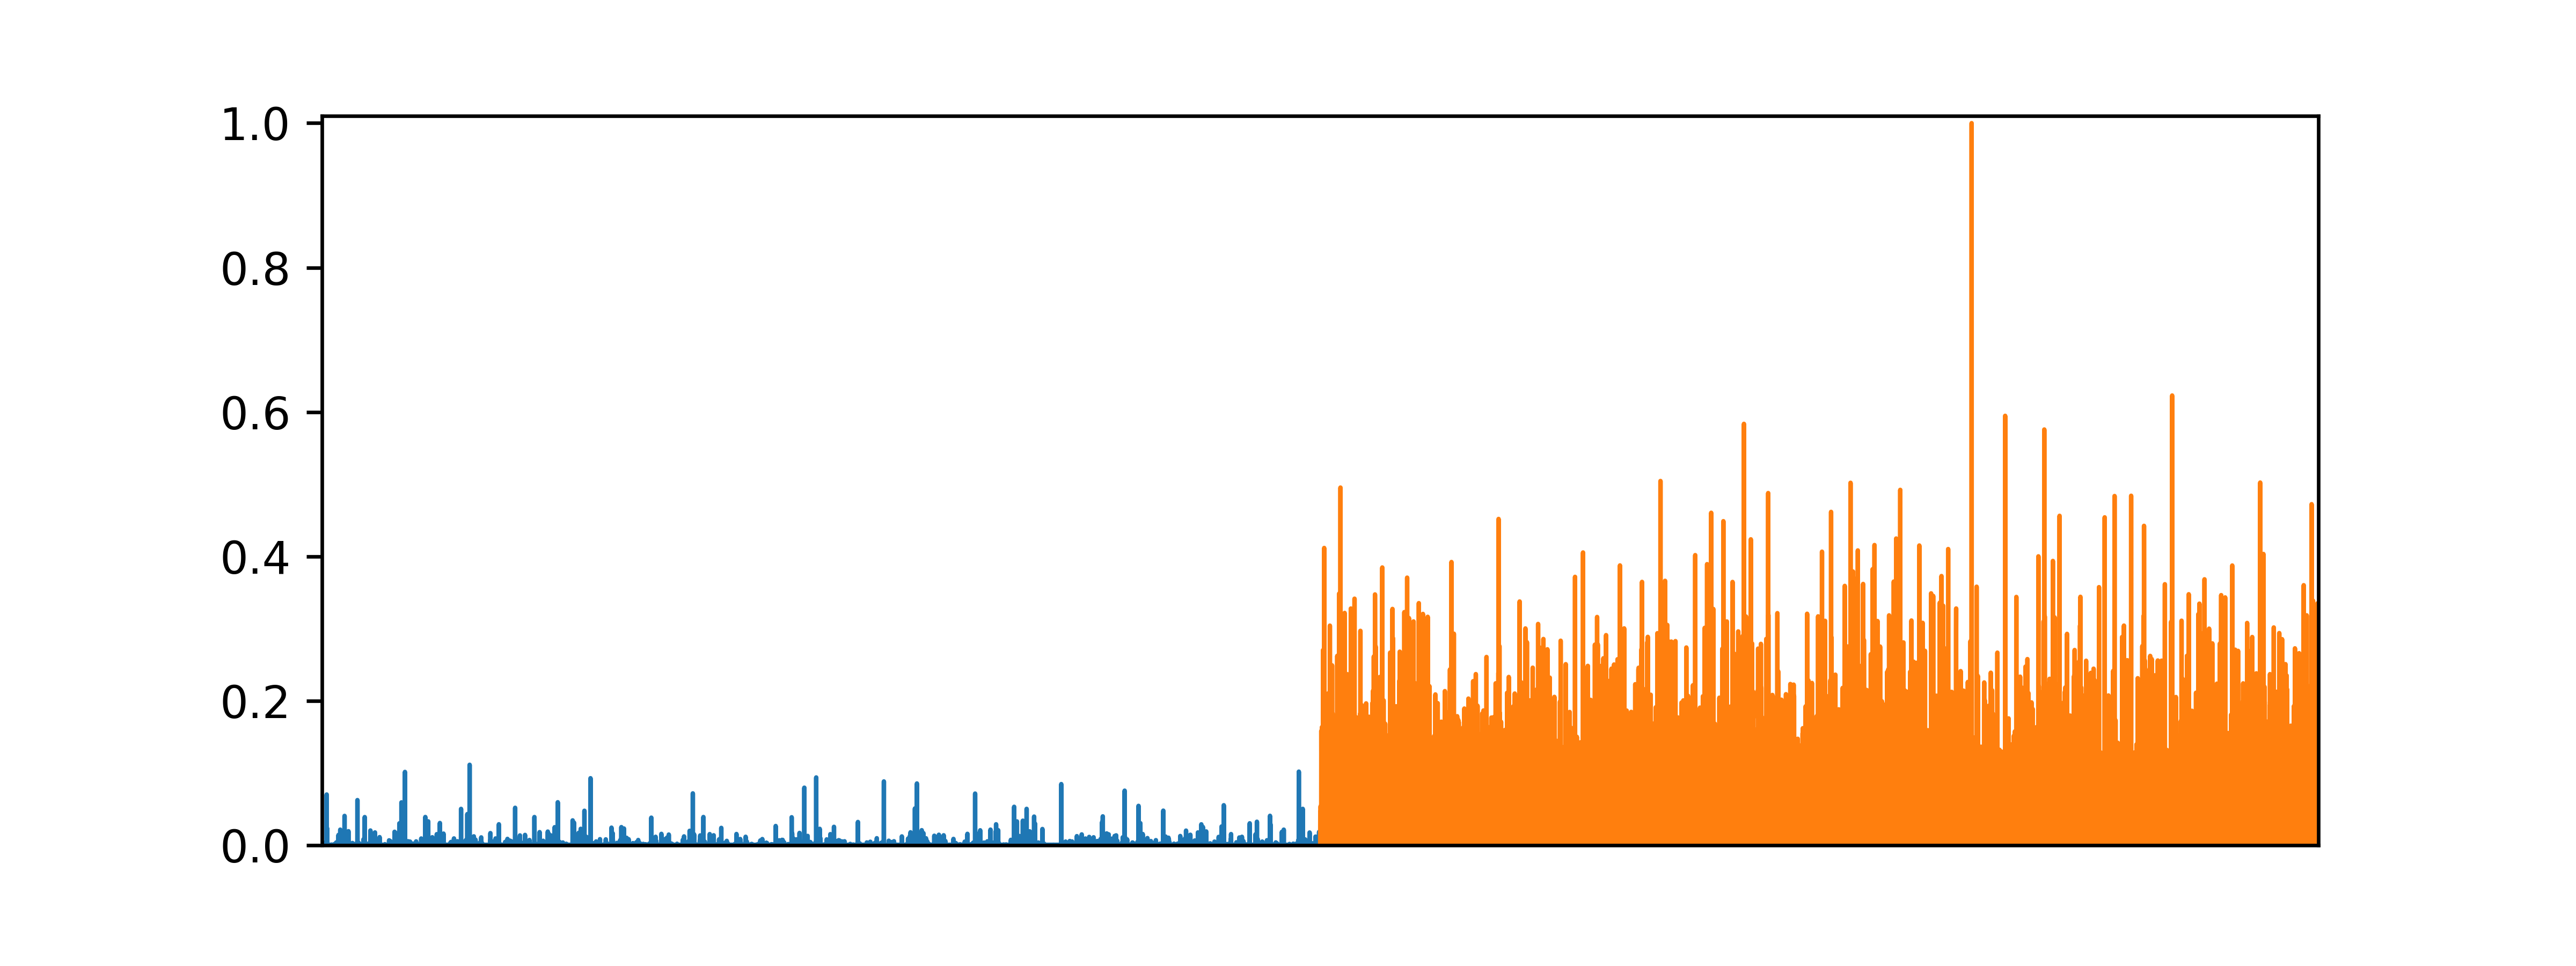
\includegraphics[height=3cm,trim=1.5cm 0.0cm 0.0cm 0.7cm,clip]{post_ae_features.png}} \\
    \subcaptionbox{Deep-level features}[.49\linewidth]{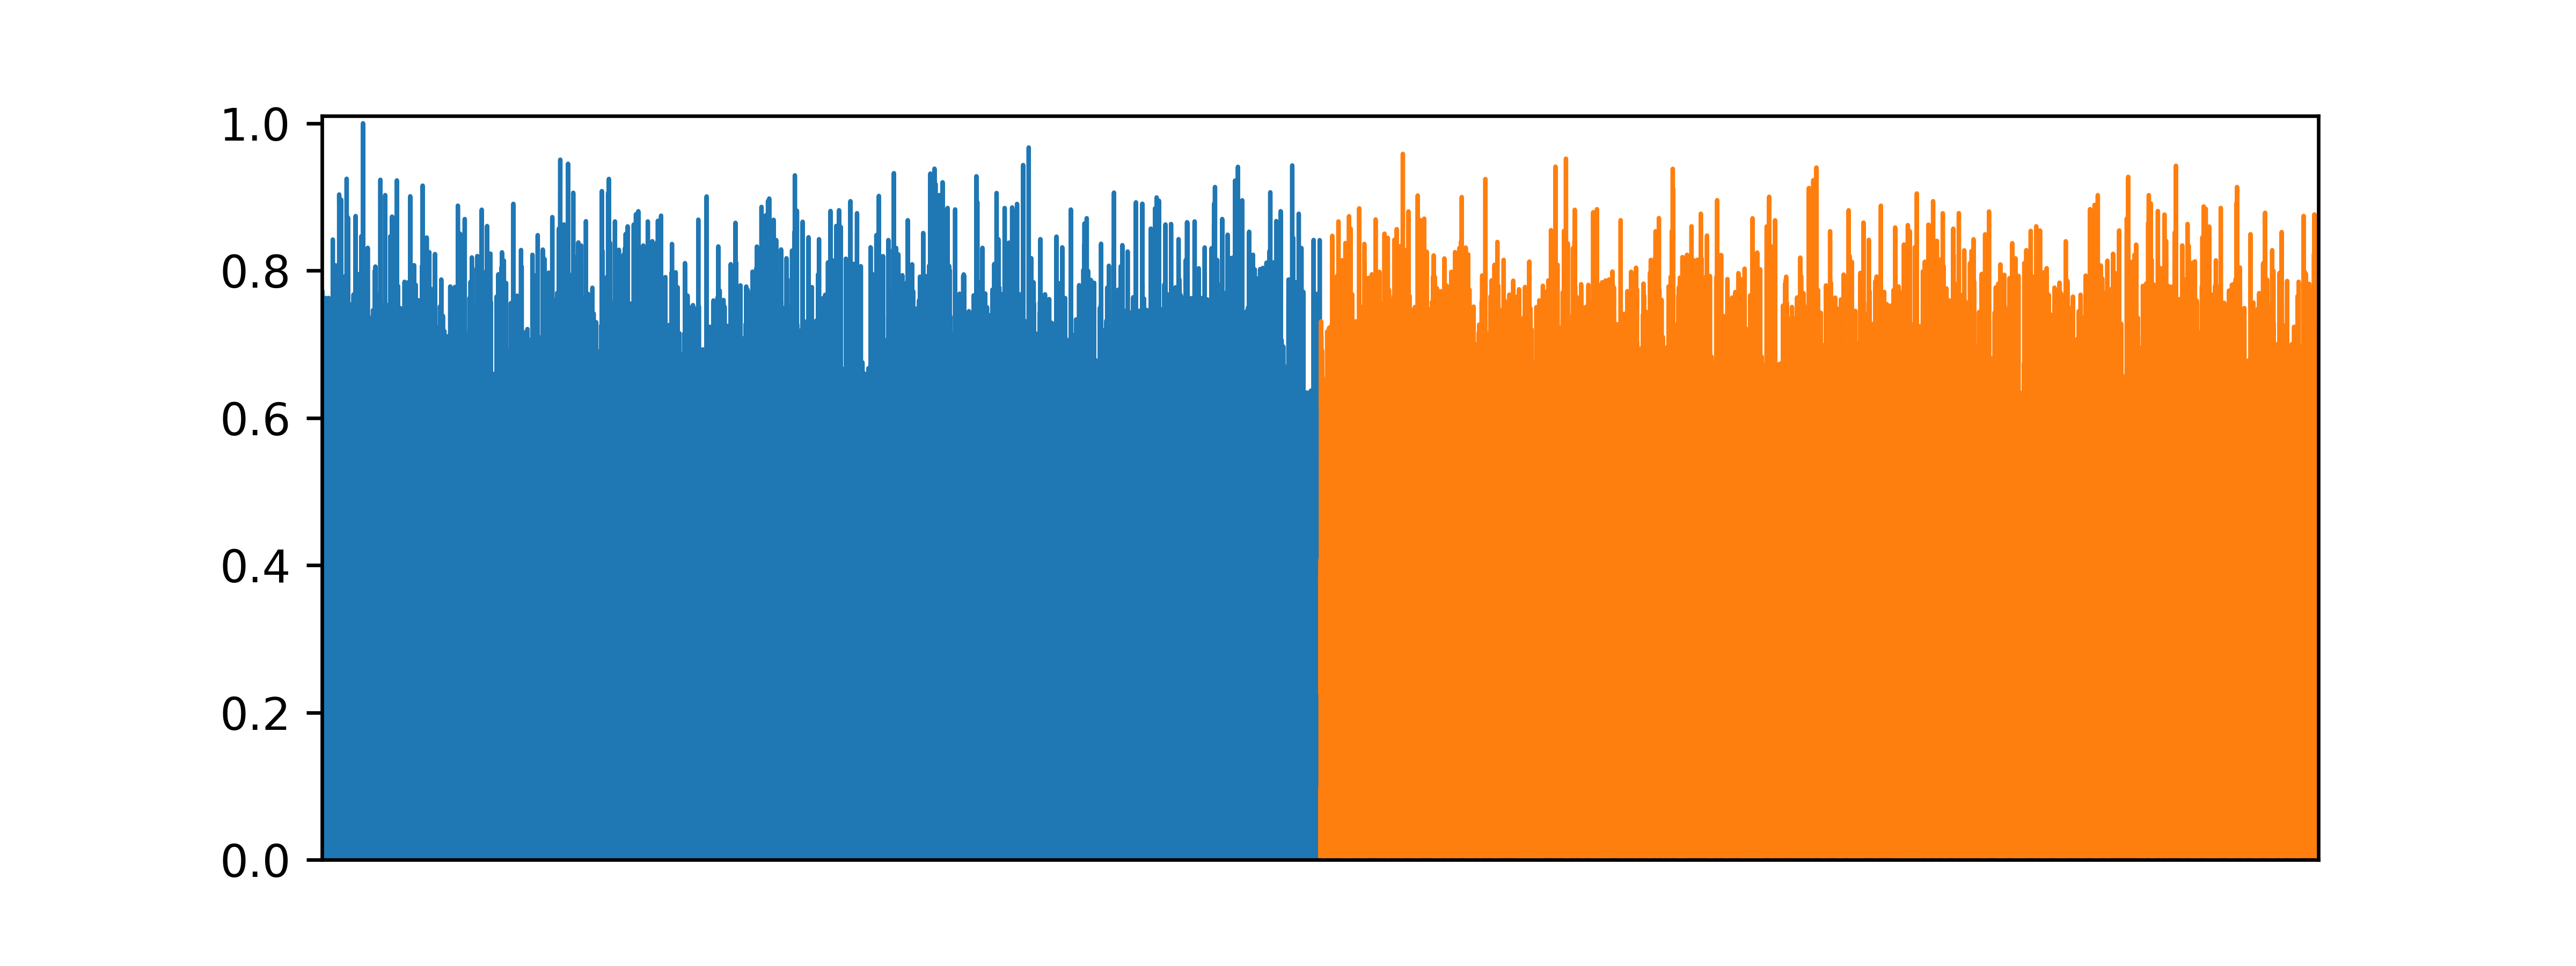
\includegraphics[height=3cm,trim=1.5cm 0.0cm 0.0cm 0.7cm,clip]{pose_ae_features_bad.png}} 
    % \subcaptionbox{Images reconstruction}[.49\linewidth]{\includegraphics[height=3cm,trim=1.5cm 0.0cm 0.0cm 0.7cm,clip]{../figures/pre_ae_features_recon.png}}
    \caption{Negative Log Likelihood (scaled to one) without (a), with (b) weighting based on the low-level features and with (c) weighting based on the deep-level features.
    In-distribution: CIFAR-10 (blue). OOD: ImageNet-resize (orange).
    Note the better separation in (b).}
     \label{Fig:ll}
\end{figure}
% In order to evaluate the reconstruction features, we replaced the proposed low-level features with either 
deep-level features. %, or the image and its reconstruction.
In~\autoref{Fig:ll}, we can see not only that the weighting based on reconstruction of low-level features (b) is better (\ie, achieves better separation) using either no weighting (a) or weighting based on reconstruction of deep-level features (c) but also that the weighting based on reconstruction of deeper features deteriorates the performance (\ie, is even worse than using no weighting). Thus the choice of low-level features is the  optimal for our use case.


\section{Datasets}
In the paper we have used several datasets:
\begin{itemize}
    \item ImageNet~\citep{Deng:CVPR:2009:imagenet}, which contains a large set of images of various categories. The curators of ImageNet do not hold the copyright of all the images,
     and the usage of that dataset is governed by the terms of the ImageNet license https://www.image-net.org/download.php.
     \item CIFAR10 and CIFAR100~\citep{Krizhevsky:Citeseer:2009:Cifar}
     (datesets of  32 x 32 RGB images).
     \item LSUN~\citep{Yu:arxiv:2015:lsun}.
     \item MNIST~\citep{Lecun:1998:mnist} (an image dataset of handwritten digits in which each instance consists of a 28x28 gray-scale image). 
     \item Omniglot~\citep{Lake:Science:2015human}, under the MIT license.
\end{itemize}

. 



\section{Implementation and Hardware Details}
\subsection{Implementation Details}
We have implemented our model using PyTorch~\citep{Paszke:NIPS:2019:Pytorch},
with the aid of several useful frameworks: PyTorch-Lighting~\citep{Falcon:github:2019:pytorch},
PyTorch Metric Learning~\citep{Musgrave:arxiv:2020pytorch}. For the DenseNet~\citep{Huang:2017:densely} implementation,
we have modified the model implementation from https://github.com/andreasveit/densenet-pytorch.
For the WideResnet28~\citep{Zagoruyko:arxiv:2016:wide} implementation, we have modified the model implementation from~\citep{Zaeemzadeh:CVPR:2021:out}.

\subsection{Hardware details}
All our experiments were done using a single NVIDIA \emph{Tesla P100} card, with the exception of the WideResNet experiments, which were done using a single NVIDIA \emph{RTX3090} card.


\section{An Intuitive Explanation for the Effect of the Overall Proposed Loss}

Recall, \eg, from Figure 4d in the paper, that the empirical effect of the overall loss is not only creating small isotropic Gaussians that are far from each other
but also forming a large empty area between them. In this section we provide some intuition behind this behavior which was consistent throughout our experiments. 
\\\\
For simplicity, suppose that there are only 5 classes and that each class consists of a single example. Let us denote the examples, as represented in a 2D latent space, by $\bmu_1$, $\bmu_2$, $\bmu_3$, $\bmu_4$ and $\bmu_5$. Now consider the following configuration. $\bmu_1=(-1,0)$, $\bmu_2=(0,-1)$, $\bmu_3=(1,0)$, $\bmu_4=(0,1)$, and $\bmu_5=(0,0)$. Here, $\bmu_5$ is at a relatively-small distance from each of the other 4 points. Moving $\bmu_5$ elsewhere would thus yield an improvement in terms of the distancing loss. In fact, a simple calculation (together with the fact that the hypotenuse is the longest side of a right-angled triangle) will show that moving $\bmu_5$ by some small epsilon in \emph{any} direction from $(0,0)$ will improve (in effect, decrease) the distancing loss.
Thus, the central region between the clusters remains effectively empty and the points will move away from it.
% Moreover,they move
\\\\
{Note however, that in our case all clusters are initialized in the center of the dataset (assuming random intialization of the latent space), thus they move simultaneously outwards, pushing away from the center of the latent space and} 
 in different directions to maximize the inter-cluster distances (if two clusters were to move together in the same direction, they would be too close to each other, incurring a penalty). Effectively, this creates a sphere-like shape (empirically, the center of that sphere tends to coincide with the origin of the latent space). 
For example, when the five points are placed on a circle in some radius at the angles (in degrees) $\set{0,72,144,216, 288}$ then each point is close to only two other points, while its distances from the others are larger. 
% Thus, in terms of the distancing loss the situation is much better when compared to the aforementioned original configuration.
{Thus, in terms of the distancing loss the penalty is smaller when compared to the
aforementioned original configuration.}
\\\\
Now, in practice cluster will of course usually contain many points, not just a single one. However, the KL loss pushes each cluster to be small and isotropic, and thus effectively behaving like a single point so the informal analysis above still holds. In contrast, without the KL loss, and due to the varying and elongated shapes of the clusters, the metric losses by themselves do not suffice for obtaining that effect.

\section{Details of the Auto-Encoders}
During the test phase of \textbf{VMDLS}, we use a pre-trained Auto-Encoder to reconstruct the images,
and use the difference between the shallow features of the reconstructed image and the original one, in order to use it as weighting during the likelihood-based decision.
The Auto-Encoders we have used are fairly simple and standard:
For CIFAR10 and CIFAR100 experiments we have used a ResNet18-based AE, as implemented by~\citep{Falcon:github:2019:pytorch}.
For the MNIST experiment we have used a simple convolutional AE, which consists of 5 convolution layers, each followed by a ReLU activation function and a pooling layer.
The exact implementation of the AEs is available in our publicly-available code. 

%\clearpage
% \small
% \bibliographystyle{ieee}
%\bibliographystyle{ieee_fullname}
% \bibliographystyle{abbrvnat}
\bibliography{refs}
%\bibliography{my_refs}


\end{document}
